\chapter{Discussion and future outlook}\label{ch:outlook}
To conclude this thesis, we shall summarise the results we have presented, discuss the potential implications\lb{Only say this if I actually do discuss implications. Otherwise need a more correct way of describing my discussion of things like how to choose \(\sigma\).}, and highlight several avenues for further extensions and applications.

In \Cref{ch:linear_theory}, we provided an \emph{explicit} bound on the error between the solution of a nonlinear stochastic differential equation and an easily computable linearisation approximation, building upon previous studies \citep{Blagoveshchenskii_1962_DiffusionProcessesDepending,FreidlinWentzell_1998_RandomPerturbationsDynamical,Sanz-AlonsoStuart_2017_GaussianApproximationsSmall}.
The linearisation approximation is used across many different applications and contexts \citep[e.g.]{Jazwinski_2014_StochasticProcessesFiltering, Sanz-AlonsoStuart_2017_GaussianApproximationsSmall,KaszasHaller_2020_UniversalUpperEstimate,ArchambeauEtAl_2007_GaussianProcessApproximations}, but often without sound mathematical justification\lb{strong statement}.
The theory applies to fully non-autonomous SDEs with multiplicative noise and a random initial condition.
Our bound is written in terms of the scale of the ongoing noise (that is, a scaling of the diffusivity coefficient) and a measure of the uncertainty in the initial condition using the \(L_r\)-norm.
A comparison in \Cref{sec:comparison} suggests that our bound on the moments is tighter than implied by the gold standard \citep{Sanz-AlonsoStuart_2017_GaussianApproximationsSmall} in the literature.
Unlike the bounds\lb{Strong statement} in other literature \citep[e.g.]{Blagoveshchenskii_1962_DiffusionProcessesDepending,FreidlinWentzell_1998_RandomPerturbationsDynamical}, by explicitly identifying the dependence of our bound on when the noise in the SDE is multiplicative and the drift nonlinear, we were also able to highlight two application-relevant special cases: when the initial condition is fixed, and when it is Gaussian.
We also provided an explicit characterisation of the distribution of the solution to the linearised SDE, enabling efficient approximation of the original nonlinear SDE using solutions to the corresponding deterministic equation, whereas previously special cases of these computations were dispersed across other literature \citep[e.g.]{Jazwinski_2014_StochasticProcessesFiltering,Sanz-AlonsoStuart_2017_GaussianApproximationsSmall,SarkkaSolin_2019_AppliedStochasticDifferential}.

Our next contribution was to provide theoretical and computational extension to the ``stochastic sensitivity'' tools introduced by \citet{Balasuriya_2020_StochasticSensitivityComputable}.
Stochastic sensitivity was hitherto derived as the variance of an unknown limiting distribution and could only be computed in two spatial dimensions; we established that stochastic sensitivity, in any number of dimensions, is computable as the operator norm of the covariance matrix of the linearised SDE.
We have also established that the limiting distribution in question is Gaussian, which may provide insight into properties of stochastic sensitivity as a means of uncertainty quantification in any model (not just in the fluids context) where an $ n $-dimensional state variable evolves according to a ``best available'' model.
This extension opens stochastic sensitivity to a much broader range of applications, which we discuss throughout this chapter.

With three example SDEs in \Cref{ch:linear_numerics}, we validated the form of our theoretical error bound and demonstrated heuristically that, in the limit of small noise, the solutions approach the approximate distributions computed by solving the linearised equivalents.
In particular, we found that the strong error scales with the initial uncertainty and ongoing uncertainty exactly as predicted.
Thus, we have provided a rigorous (in the sense of a bound and a limit) justification for using such approximations when the noise in the model is small, and a framework for rapid computation of the first two moments of the linearisation.

However, in \Cref{ch:gmm} we highlighted that there are limitations to using Gaussian approximations, most notably that they cannot capture features such as skew and multimodality in the solution distribution.
To overcome these limitations while still taking advantage of the computationally efficiency of the linearisation approximation, we proposed an \emph{ad hoc} algorithm that uses a splitting process to approximate SDE solutions with a Gaussian mixture model.
Each component of the mixture model arises from a solution of the SDE linearised about a \emph{different} deterministic trajectory, which means that we can capture uncertainty in different regions.
With a simple propagation-splitting procedure, the algorithm is able to capture multimodality, skewness, and other departures from Gaussianity in the solution to a stochastic differential equation, providing an approximation that improves upon a single Gaussian component but does not require the computational expense of bulk simulation.
Another advantage of this algorithm is that it provides a probability density function that can be evaluated analytically, as opposed to stochastic samples which require an additional step to construct a density function estimate.
Our aim throughout was to outline the algorithm and demonstrate the potential of it on several simple implementations, rather than explore the specifics of each step or analysing mathematically.
Instead, we discuss several directions for further refinement of this algorithm in \Cref{sec:gmm_extensions} and leave this for future work.

In \Cref{ch:appls}, we applied the developments of the previous chapters to two data-driven examples arising from completely different settings.
Our first application was to a 2-dimensional model for the motion of a drifter on the surface of the Gulf Stream, in the North Atlantic Ocean, constructed from interpolated satellite-measured velocity data.
\td{Summarise Gulf Stream results}
The mixture model showed highly promising results on this example trajectory; with only 2 splits and 25 components, the algorithm was able to closely recreate the highly non-Gaussian distribution.
\td{Summarise epi stuff}


There are some similarities between our approaches and tools used in population processes and compartmental modelling, linked by the diffusion limit of a compartmental model summarised in \Cref{sec:epi_limits}.
For example, the covariance matrix of the limit can measure the variation not accounted for when using the deterministic limit alone \citep{PollettEtAl_2010_ModellingPopulationProcesses}.
This is a similar idea to stochastic sensitivity, which quantifies the uncertainty in using predictions from a deterministic differential equation.
However, these ideas are novel in the broader context of dynamical systems, and in particular in the field of Lagrangian prediction and coherent structure extraction.
\td{Definitely need to word this better, trying to say that although some similar ideas are floating around in epi, we have novel applications and get to it from a completely different avenue. The consistency is a good thing that we've verified.}




\section{Selecting the diffusion matrix \(\sigma\)}
\note{Discussion about selecting \(\sigma\), with a short review of some of the literature out there. Should this be its own section??}
A powerful advantage of our framework is that the diffusivity matrix \(\sigma\) is permitted to vary spatio-temporally, allowing for multiplicative noise.
Multiplicative noise is often ignored in practice, due to difficulties in working with analytically (see, for instance, the prior lack of rigorous justification of linearisations when the noise is multiplicative) and generating numerical realisations efficiently (e.g. the review by \cite{MoraEtAl_2017_StableNumericalScheme}).
Despite these challenges, multiplicative noise is often necessary in practice \citep{Sura_2003_StochasticAnalysisSouthern,KamenkovichEtAl_2015_PropertiesOriginsAnisotropic,anymore?}.
For example, \citet{SuraEtAl_2005_MultiplicativeNoiseNonGaussianity} showed that multiplicative noise on linear dynamics can model departures from Gaussianity observed in climate statistics, as opposed to nonlinear dynamics with only additive noise.
The spatiotemporal dependence of \(\sigma\) can also capture experimental and observational considerations that are otherwise ignored in the deterministic model, such as cloud cover when using satellite measurements or nonuniform uncertain across the field of view of a camera \citehere.
This does raise the question, however, of exactly \emph{how} to specify \(\sigma\), particular when the aim is to measure uncertainty in a model that is only specified deterministically\lb{Word this better}.
If there is no \emph{a priori} knowledge about the spatiotemporal nature of the noise, then the default choice of \(\sigma \equiv I\) addresses a generic situation \citehere.
There are many different methods for estimating \(\sigma\) directly from observed data, e.g. via statistical estimation \citep{CotterPavliotis_2009_EstimatingEddyDiffusivities}  or the Bayesian inference approach of \citet{YingEtAl_2019_BayesianInferenceOcean}.
Coupling these approaches with the approximation here could provide a complete and practical framework for constructing a Gaussian approximation from observed trajectory data only, without the need to directly specify the diffusion matrix as part of the model.
In oceanography, a common approahc is to specify the diffiusion term as part of a physics-informed model \citep{BerloffMcWilliams_2002_MaterialTransportOceanic}.
\td{Definitely more to say here. Informed by physics, models, etc?? Any cirtations for atmospheric papers}
\td{Refer to how we choose it in epi examples??}
We must emphasise, however, that in general the specification of the diffusion term is an open question and depends on the specifics of the situation and modelling choices.

\section{Fixed states and boundary conditions}
\td{Some sort of overview of boundaries ??}

boundary conditions can be informed by physical aspects of the model


Enforcing boundary conditions is ani additional challenge when working with stochastic differential equations
\td{Back this up with sources}
An absorbing boundary can be accounted for by setting both the drift and diffusivity in the stochastic differential equation to zero on the boundary.
However, such adjustments will often violate the requirements of smoothness in these terms set out in \Cref{hyp:smooth}.
More generally, one can stochastic differential equations with boundary conditions, and it can be shown that such SDEs do in fact have unique solutions; an introduction to the formal treatment of stochastic differential equations with boundary conditions is provided by \citet{Pilipenko_2014_IntroductionStochasticDifferential}.
% However, the presence of boundary conditions is beyond the scope of this thesis and we will instead ensure that we choose initial conditions and values so that the impact of boundaries is negligible.

An \(n\)-dimensional Gaussian density has support on the entirety of \(\R^n\), meaning that for \emph{any} sensible non-empty region in \(\R^n\), there is a non-zero probability that a random variable following a non-degenerate Gaussian distribution takes a value in that region.
As we demonstrated on the SIR example in \cref{fig:sir_gauss_rels}, this property means that a Gaussian approximation, such as that arising from the linearisation of an SDE, cannot capture boundaries.

The Gulf Stream example in \Cref{sec:appl_ocean} provides another example of boundary conditions.
Firstly, the subset of altimetry data that we used was only available on a finite spatial region, which is almost always the case in data-driven models.

When generating realisations, a n\"aive approach to handle these boundaries is to discard any trajectories that leave the spatial domain.

In our examples, we avoided this complication by ensuring that the target densities and the evolution of solution trajectories were sufficiently far from the boundaries so that the probability that a solution or the resulting approximations were nearby was negligible.

\begin{itemize}
	\item Boundary conditions can be informed by physical aspects of the model, e.g. expecting that a variable must be non-negative or the presence of boundaries, or limitations of the underlying data, e.g. only available on a finite set.
	\item We saw some examples of this - the Gulf Stream dataset was only available on a finite spatial grid, and there was land which was both missing data and . Epi examples - population sizes are non-negative, and once we scaled to approximate with the diffusion limits, the variables were confined to \([0,1]\).
	\item Enforcing these boundary conditions on a stochastic differential equation is difficult, since stochasticity messes things up.
	\item A couple of standard options are absorbing boundary conditions - the drift and diffusion are set to zero, which means that the boundary acts as a fixed point of the system.
	\item Another option is a reflecting boundary condition, where solution trajectories are `pushed away' from the boundary, possibly with some additional conditions - see \citet{Pilipenko_2014_IntroductionStochasticDifferential} for details.
	\item Can we handle these cases in our theory??
	\item Big limitation of Gaussian approximations is that they cannot account for these boundary conditions. Saw this in \Cref{fig:sir_gauss_rels}. We ignored the issue here by ensuring that we were far away from boundaries.
	\item In epi modelling, generally accepted as a significant limitation of the diffusion limimt
	\item This extends to our GMM, which suffers from the same issue.
	\item Naive approach when simulating is to discard any violating realisations - could adopt a similar idea and either truncate or take the negative mass and assign to the boundaries.
	\item For example, in the epidemic models, any zero state is an absorbing boundary, so any mass that ends up there should remain there - take the negative mass and put it at zero?
	\item Perhaps show a figure or two doing exactly this with the SIR model??
	\item In general, enforcing boundary conditions on stochastic differential equations is difficult and an area of ongoing research.
	\item Worth commenting on fixed states? Fun question - what happens if we initialise our linearisation about a fixed state??
\end{itemize}


% \begin{figure}
% 	\centering
% 	\begin{subfigure}{0.49\textwidth}
% 		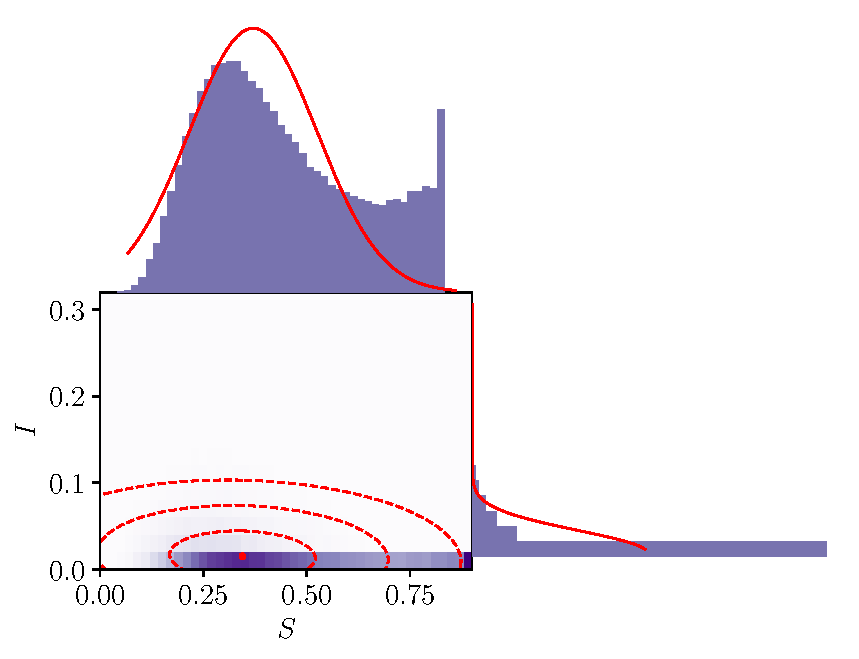
\includegraphics[width=\textwidth]{chp06_applications/figures/sir/sir_pairwise_50_truncated}
% 		\caption{Truncation}
% 	\end{subfigure}
% 	\begin{subfigure}{0.49\textwidth}
% 		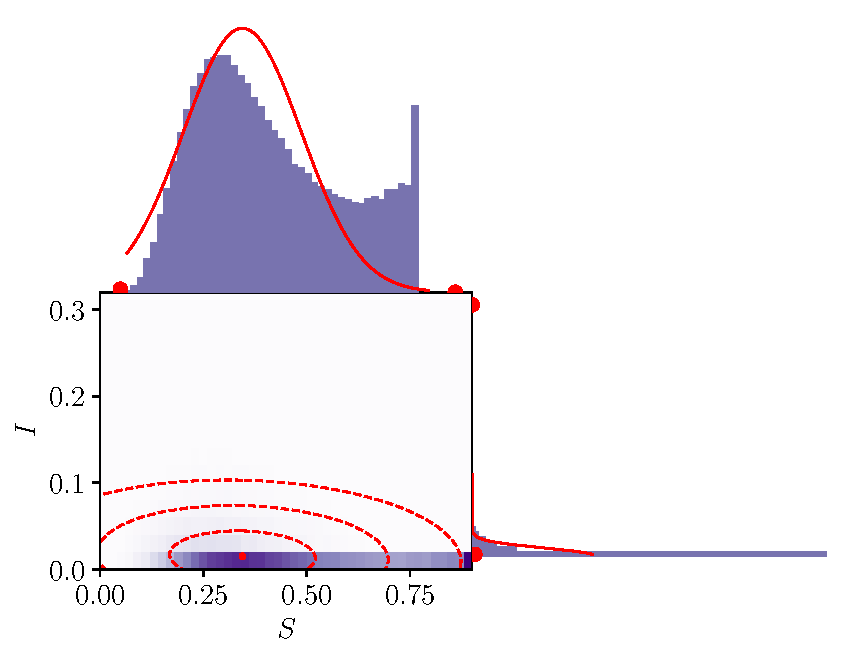
\includegraphics[width=\textwidth]{chp06_applications/figures/sir/sir_pairwise_50_adjusted}
% 		\caption{Assigning negative mass to zero}
% 	\end{subfigure}
% 	\caption{}
% 	\label{fig:}
% \end{figure}



\section{Applications to population processes}
In the limit of large population sizes, a deterministic ordinary differential equation and linear stochastic differential equation arise from certain population processes, despite these processes being discrete.
A population process is \emph{density dependent} (in the sense of \citet{Kurtz_1970_SolutionsOrdinaryDifferential}) if there is a parameter \(N\) such that
\begin{equation}
	q\!\left(n, n+l\right) = Nf\!\left(\frac{n}{N}, l\right),
	\label{eqn:ctmc_dens_dep}
\end{equation}
where \(f\) is a suitable function and \(n, n+l \in \mathcal{S}\).
Typically, \(N\) is related to the size of the system and \(n / N\) is a population density.
The condition in \cref{eqn:ctmc_dens_dep} states that the transition rates of the process \(X_t\) depends on \(X_t\) itself only through the density \(X_t / N\).

Let \(Y_t^{(N)}\) describe the \(n\)-dimensional density process, i.e. with \(i\)th element \(X_t^{(i)} / N\).
Theorem 3.1 of \citet{Kurtz_1970_SolutionsOrdinaryDifferential} establishes that in the large population limit \(N \to \infty\), the density process \(Y_t^{(N)}\) converges in probability to a deterministic trajectory \(Y_t^{(\infty)}\) solving the ODE
\begin{equation}
	\dod{Y_t^{(\infty)}}{t} = Q\!\left(Y_t^{(\infty)}\right), \quad Y_0^{(\infty)} = X_0 / N,
	\label{eqn:ctmc_dens_dep_ode}
\end{equation}
where
\[
	Q\!\left(y\right) = \sum_{\substack{l \in \R^n \\ l \neq 0,\, y + l \in \mathcal{S}}}{l f\!\left(y, l\right)}.
\]
For large \(N\), the density process has small variation and is ``close'' to the deterministic solution to \cref{eqn:ctmc_dens_dep_ode}.
This result is analogous to that for small noise SDEs; the solution to a stochastic differential equation formally converges to that of a deterministic system (involving only the drift term) in the limit of small noise, which is a result established by large deviations principles \citep[e.g]{FreidlinWentzell_1998_RandomPerturbationsDynamical}.

\citet{Kurtz_1971_LimitTheoremsSequences} then established a stronger result, showing that the variation of the density process about this deterministic limit is captured by an It\^o diffusion.
Define the scaled process
\[
	Z_t^{(N)} = \sqrt{N}\left(Y_t^{(N)} - Y_{t}^{(\infty)}\right),
\]
then Theorem 3.5 of \citet{Kurtz_1971_LimitTheoremsSequences} proves that \(Z_t^{(N)}\) converges in distribution (weakly) to an It\^o diffusion \(Z_t^{(\infty)}\) solving
\begin{equation}
	\dif Z_t^{(\infty)} = \nabla Q\!\left(Y_t^{(\infty)}\right) Z_t^{(\infty)}\dif t + G\!\left(Y_t^{(\infty)}\right)\dif W_t, \quad Z_0^{(\infty)} = 0,
	\label{eqn:ctmc_dens_dep_sde}
\end{equation}
where \(W_t\) is an \(n\)-dimensional Wiener process and the \(n \times n\) diffusion matrix \(G\) is such that
\begin{equation}
	\left[G\!\left(y\right)G\!\left(y\right)^{\T}\right]_{ij} = \sum_{\substack{l \in \R^n \\ l \neq 0,\, y + l \in \mathcal{S}}}{l_i l_j f\!\left(y,l\right)}
	\label{eqn:ctmc_dens_dep_sde_diff_cond}
\end{equation}
Any choice of diffusion matrix \(G\) such that \cref{eqn:ctmc_dens_dep_sde_diff_cond} is satisfied will result in a statistically identical diffusion process \(Z_0^{(\infty)}\).

The limiting SDE \cref{eqn:ctmc_dens_dep_sde} is equivalent to the unscaled SDE
\begin{equation}
	\dif L_t^{(N)} = \left[Q\!\left(Y_t^{(\infty)}\right) + \frac{1}{\sqrt{N}} \nabla Q\!\left(Y_t^{(\infty)}\right)\left(L_t^{(N)} - Y_t^{(\infty)}\right)\right]\dif t + \frac{1}{\sqrt{N}}G\!\left(Y_t^{(\infty)}\right)\dif W_t,
	\label{eqn:ctmc_sde_lin_lim}
\end{equation}
which is a linearisation of the nonlinear SDE
\begin{equation}
	\dif \hat{Y}^{(N)}_t = Q\!\left(\hat{Y}^{(N)}_t\right)\dif t + \frac{1}{\sqrt{N}}G\!\left(\hat{Y}_t^{(N)}\right)\dif W_t
	\label{eqn:ctmc_sde_lim_nonlin}
\end{equation}
about the deterministic limit \(Y_t^{(\infty)}\).
There is intuition behind the choices of drift and diffusion in \cref{eqn:ctmc_sde_lim_nonlin}.
For sufficiently large \(N\), the drift term \(Q\) captures the average (macroscopic) behaviour of the density process.
The diffusion term captures the microscopic behaviour resulting from individual transition events, and the uncertainty in this is parameterised with the Wiener process \(W_t\).




\td{Explain how this is analogous to the proceeding work}
However, a key difference is that in the SDE linearisation procedure, we start from a continuous state-space process and arrive at a continuous state-space process in the limit.
Whereas, in the CTMC diffusion limit, the converging process is on a \emph{discrete} state-space and the limit is on a continuous one.




Thus, we expect that the mixture model algorithm we have described may find a place in moderate-population compartmental models, where the population is large enough to be ``reasonably'' approximated by the continuum and SDE equations, but small enough to exhibit non-Gaussian behaviour.
Regardless, our error bound derived in \Cref{ch:linear_theory} still has a place in this literature.





\section{Further theoretical developments}
In this section, we briefly postulate three extensions to the theoretical results presented in \Cref{ch:linear_theory}.



\subsection{Non-Gaussian noise processes}\label{sec:disc_levy}
Throughout this thesis, we have considered It\^o stochastic differential equations driven by the canonical Wiener process, and so we are assuming that the noise in our system is white (zero temporal correlation) and Gaussian.
However, when modelling physical systems (e.g. climate and oceanographic models), there is observational evidence to suggest the underlying noise process may be better formulated as a more general L\'evy process \citep{Ditlevsen_1999_ObservationAstableNoise, Viecelli_1998_PossibilitySingularLowFrequency}.
A L\'evy process satisfies the same properties as the Wiener process, but without Gaussian increments \citep{Applebaum_2004_LevyProcessesStochastic}, and can capture departures from Gaussianity, such as skew and heavy-tailedness, in the ongoing noise process.
A majority of the results for stochastic differential equations hold for when the Wiener process is replaced by a L\'evy process \citep{Applebaum_2004_LevyProcessesStochastic}.

\citet{GottwaldMelbourne_2013_HomogenizationDeterministicMaps} show that stochastic differential equations driven by L\'evy processes arises as the limit of \td{quickly summarise this paper}
\citet{PenlandEwald_2008_ModellingPhysicalSystems} provide \td{Summarise}

There is scope to determine whether the theory presented in \Cref{ch:linear_theory}, and importantly the computability of the linearisation solution, can be generalised to stochastic differential equations driven by arbitrary L\'evy processes.
If we replace the Wiener process in \Cref{thm:main}, the proofs in \Cref{sec:paper_proofs} will still hold as they rely on results for general It\^o integrals and square-integrable stochastic processes.
This would show that such a solution, for small noise, can be approximated by an It\^o integral of a deterministic function (i.e. \cref{eqn:linear_sol}) with respect to the driving process.
The applicability of this approximation then depends upon how easily this integral can be evaluated, without having to numerically solve the original stochastic differential equation.



\subsection{Pursuing higher order terms}
The linearisation approximation introduced in \Cref{ch:linear_theory} that underpins the work in this thesis equivalently arises by considering a formal power-series expansion of the SDE solution.
That is, given the solution \(y_t^{(\epsilon)}\) to a small-noise SDE
\begin{equation}\label{eqn:y_sde_outlook}
	\dif y_t^{(\epsilon)} = u\!\left(y_t^{(\epsilon)}, t\right)\dif t + \epsilon \sigma\!\left(y_t^{(\epsilon)}, t\right)\dif W_t,
\end{equation}
one can consider a power-series expansion in \(\epsilon\)
\begin{equation}\label{eqn:y_sde_expans}
	y_t^{(\epsilon)} = z_t^{(0)} + \epsilon z_t^{(1)} + \epsilon^2 z_t^{(2)} + \dotsb + \epsilon^m z_t^{(m)} + \dotsb,
\end{equation}
where the coefficients \(z_t^{(0)}, z_t^{(1)}, z_t^{(2)}, \dotsc\) are themselves stochastic processes.
Such expansions are considered by \citet{Blagoveshchenskii_1962_DiffusionProcessesDepending}, who found generic bounds for the expected distance between the solution to \cref{eqn:y_sde_outlook} and truncations of \cref{eqn:y_sde_expans}.
The linearised SDE corresponds to truncating \cref{eqn:y_sde_expans} to the \(m = 1\) term.
Specifically, in finding the solution \(l_t^{(\epsilon)}\) we implicitly established that \(z_t^{(0)} = F_0^t\!\left(x_0\right)\), the deterministic flow map, and \(z_t^{(1)}\) can be expressed as the It\^o integral of a deterministic function (i.e. compare \(z_t^{(0)} + \epsilon z_t^{(1)}\) with \cref{eqn:linear_sol})\lb{Just need to check that I'm consistent with previous notation. Initial condition?}.
We expect that including more terms when truncating \cref{eqn:y_sde_expans} will result in a `better' approximation of the original SDE solution, in the same fashion as a Taylor expansion of a deterministic function.
It is worth noting that this is not immediately apparent from the results of \citet{Blagoveshchenskii_1962_DiffusionProcessesDepending} and \citet{FreidlinWentzell_1998_RandomPerturbationsDynamical}\lb{check that this is actually the case before claiming it. Probably not actually the case - think about scaling with \(\epsilon\)}.
An obvious extension to our theoretical results would be to higher order expansion, where we look to continue building upon \citet{Blagoveshchenskii_1962_DiffusionProcessesDepending,FreidlinWentzell_1998_RandomPerturbationsDynamical} to provide explicit bounds on the distance between the SDE solution and a truncation.
From a practical perspective, this also raises a question of whether the higher-order terms can be computed to provide a more accurate approximation of nonlinear SDE solutions.
However, the higher order coefficients obey nonlinear stochastic differential equations which cannot in general be solved analytically.
For example, by performing Taylor expansions of the coefficients of \eqref{eqn:y_sde_outlook} and rearranging, the second-order term \(z_t^{(2)}\!\left(\epsilon\right)\) is shown to solve
\[
	\dif z_t^{(2)}\!\left(\epsilon\right) = \begin{multlined}[t]
		\left[\frac12 z_t^{(1)}\!\left(\epsilon\right)^{\T} \nabla\nabla u\!\left(F_0^t\!\left(x_0\right), t\right) z_t^{(1)}\!\left(\epsilon\right) + \nabla u\!\left(F_0^t\!\left(x_0\right), t\right) z_t^{(2)}\!\left(\epsilon\right)\right]\dif t \\
		+ \nabla \sigma \!\left(F_0^t\!\left(x_0\right), t\right) z_t^{(1)}\!\left(\epsilon\right)\dif W_t
	\end{multlined}
\]
This equation is difficult to solve even numerically, due to the nonlinearity and dependence on the second derivatives of \(u\).
Thus, while there is potential to extend our \emph{theoretical} results to higher-order expansions, we expect that there would not be the sane \emph{practicality} of computation that we relied upon later in the thesis.


\subsection{The Fokker-Planck equation}
\note{Introduce FP-equation and talk about potential to link to current work.}
The Fokker-Planck equation is a partial differential equation that describes the time-evolution of the probability density function of the solution to a stochastic differential equation.
The probability density function \(\rho\) for the solution to the SDE \cref{eqn:gen_sde} at time \(t \in [0,T]\) is the solution to the corresponding Fokker-Planck equation \citep{Risken_2012_FokkerPlanckEquationMethods}
\begin{equation}
	\dpd{\rho}{t} = \frac12\nabla\cdot\nabla\cdot\left(\rho\sigma\sigma^{\T}\right) - \nabla\cdot\left(\rho u\right)
	\label{eqn:fp_eqn}
\end{equation}
subject to some initial density \(\rho\!\left(x,0\right)\) given by the distribution of the initial condition to \cref{eqn:gen_sde}.
% For a fixed and deterministic initial condition \(y_0 = x\), the corresponding initial condition to \cref{eqn:fp_eqn} is the Dirac-delta distribution centred at \(x\).
% To ensure that the solution is a valid probability density function on \(\R^n\), for any \(t \in [0,T]\), \(\rho\) must satisfy
% \begin{subequations}\label{eqn:fp_valid_pdf}
% 	\begin{align}
% 		\int_{\R^n}{\rho\left(x, t\right)\dif x} = 1, \label{eqn:fp_valid_pdf_norm} \\
% 		\lim_{x \to \infty}\rho\left(x,t\right) = 0. \label{eqn:fp_valid_pdf_limit}
% 	\end{align}
% \end{subequations}
Solving the Fokker-Planck equation provides an alternative method for finding the solution to a stochastic differential equation; rather than dealing with stochastic trajectories, we instead seek solutions to a partial differential equation.
However, the Fokker-Planck equation cannot be solved analytically except for simple cases and so is typically solved approximately.
There are typically two approaches to numerically solving the Fokker-Planck equation: either by generating many stochastic realisations by solving the corresponding SDE \cref{eqn:gen_sde} numerically and using a density estimation method \citep{Silverman_2017_DensityEstimationStatisticsa}, or by directly solving the Fokker-Planck equation with a finite-difference or finite-element scheme \citep{PichlerEtAl_2013_NumericalSolutionFokker}.
There are several practical difficulties with either approach, including:
\begin{itemize}
	\item \textbf{Dimensionality:} In high-dimensional systems, solving the Fokker-Planck equation numerically is computationally prohibitive, requiring either  a large number of stochastic samples or a fine spatial discretisation to be accurate.

	\item \textbf{Boundary conditions:} The Fokker-Planck equation is often defined on an unbounded domain with the zero-limit constraint \(\lim_{\norm{x} \to \infty}\rho\!\left(x,t\right) = 0\), which presents additional computational difficulties.

	\item \textbf{Normality constraints:} The Fokker-Planck equation must be solved with additional normality condition---the solution represents a probability density function, and so must always be bounded and integrate to 1---which enforces an additional constraint on any numerical solution.
\end{itemize}
It is generally accepted that these difficulties mean that the computational cost of solving the Fokker-Planck equation is too high in \(3\)- or higher dimensions \citep{ZhaiEtAl_2022_DeepLearningMethod,Li_2019_DatadrivenMethodSteady,AllawalaMarston_2016_StatisticsStochasticallyForced,AndersonFarazmand_2024_FisherInformationShapemorphing}.
% There has been much recent interest in developing data-driven methods for solving the Fokker-Planck equation directly \citep{ZhaiEtAl_2022_DeepLearningMethod,Li_2019_DatadrivenMethodSteady,AllawalaMarston_2016_StatisticsStochasticallyForced,AndersonFarazmand_2024_FisherInformationShapemorphing}.
Our approaches can provide analytic probability density functions, which are seen as direct approximations of the solution to the Fokker-Planck equation.
\td{Need to link our work to FP equation, and explain how this may overcome limitations}
Moreover, understanding the relationship between SDE linearisations and the Fokker-Planck equation may provide an avenue for further developing the Gaussian mixture model algorithm of \Cref{ch:gmm}.
The aim of the mixture model is to approximate the probability density function of the solution to the SDE, and so the Fokker-Planck equation may be a more appropriate framework for investigating this algorithm, as opposed to the solution-trajectory focus of the theory in \Cref{ch:linear_theory}.

\td{Implications for the advection-diffusion equation}
The Fokker-Planck equation is equivalent to an advection-diffusion equation, which in classical mechanics\lb{?} describes the spread of a passive scalar within a flow, with a spatiotemporally varying diffusion coefficient.
This connection often leads to the construction of \(\sigma\) in oceanographic models; the impact of subscale vortices is quantified via physical arguments to describe the transport of material with an advection-diffusion equation, which corresponds to a Fokker-Planck equation and therefore a stochastic differential equation.

\section{Further development of the GMM algorithm}\label{sec:gmm_extensions}
\note{Several avenues for further developing the GMM algorithm. Discuss \citet{DeMarsEtAl_2013_EntropyBasedApproachUncertainty} in more detail.}
In describing our mixture model algorithm in \Cref{ch:gmm}, we deliberately left several steps in general terms: the initialisation of the algorithm (for an arbitrary initial condition), the criterion for deciding when to split a component, and the construction and weighting of the split points.



\section{Further applications}
In \Cref{ch:appls}, we applied the Gaussian approximation and the mixture model algorithm to data-driven examples.
However, we only scratched the surface of the potential applications of this work.

Our error bound may be useful to investigate the validity of SDE linearisations in application domains such as Stochastic Parameterisation \citep{BernerEtAl_2017_StochasticParameterizationNew,Palmer_2019_StochasticWeatherClimate,LeutbecherEtAl_2017_StochasticRepresentationsModel} or Data Assimilation \citep{BudhirajaEtAl_2019_AssimilatingDataModels,ReichCotter_2015_ProbabilisticForecastingBayesian,LawEtAl_2015_DataAssimilationMathematical}, or to improve such linearisations by monitoring the skew or kurtosis.


\subsection{Lagrangian coherent structures}
\note{LCS extraction in n-dimensions. Quantifying uncertainty a la \citet{BadzaEtAl_2023_HowSensitiveAre}. Furthering \citet{Balasuriya_2020_UncertaintyFinitetimeLyapunov}, etc.}

As a recent development, stochastic sensitivity has hitherto seen limited application \citep{BadzaEtAl_2023_HowSensitiveAre,Balasuriya_2020_UncertaintyFinitetimeLyapunov,FangEtAl_2020_DisentanglingResolutionPrecision}.
We have presented a complete generalisation of these tools to arbitrary dimensions (\Cref{def:ss_Rn}), and established the connection to SDE linearisation that empowers a rapid computation (\Cref{thm:s2_calculation}).

Most traditional LCS measures are completely deterministic measures, not accounting for any uncertainty in the driving velocity field, and the sensitivity of these methods to such uncertainty has not been investigated in detail.
The robustness of several LCS methods to stochastic noise has recently been explored by \citet{BadzaEtAl_2023_HowSensitiveAre}, but via stochastic simulation and summary statistics.
In this paper we have presented a theoretical result for characterising Lagrangian trajectory uncertainty, which can be used to perform a purely theoretical analysis of such sensitivity in LCS computations.
The linearised covariance matrix and stochastic sensitivity values are computable using the flow map gradient \(\nabla F_0^t\), which is a quantity often used in LCS computation, and so can enable a rapid and convinient computation to \emph{supplement} an LCS extraction scheme\lb{This is a poorly phrased sentence. Trying to emphasise that stochastic sensitivity can complement after LCS computations.}.
\citet{Balasuriya_2020_UncertaintyFinitetimeLyapunov} provides a preliminary derivation (using the previously 2-dimensional formulation of stochastic sensitivity by \citet{Balasuriya_2020_StochasticSensitivityComputable}) of uncertainty in the finite-time Lyapunov exponent.
With the extension of stochastic sensitivity to arbitrary dimensions and the additional knowledge of Gaussianity in the relevant underlying distribution, this initial work could be formalised (e.g. in terms of statistical confidence intervals) to provide a leading-order estimate for the error in FTLE computations.

\citet{BalasuriyaEtAl_2018_GeneralizedLagrangianCoherent} provide a framework that extends the notion of a Lagrangian coherent structure to capture spatial ``regions of interset'' in the time-evolution of other quantities that are transported by, but not fully locked to, a flow.
Examples of these quantities include the concentration of pollutants, the density of an organism such as phytoplankton, temperature, and salinity in the fluid context.
In \Cref{sec:fp_eqn}, we explained how via the Fokker-Plank equation, the spread of a tracer under the advection-diffusion equation can be equivalently captured by the solution to a stochastic differential equation.
The spread of ``uncertainty'' in the stochastic formulation corresponds to the movement and dispersion of the tracer, in the sense that the probability density function of the stochastic solution is exactly the (normalised) tracer concentration.
In capturing this uncertainty and extracting spatial regions from the resulting field, stochastic sensitivity can offer insight into the spread of such tracers, and potentially be used to extract generalised Lagrangian coherent structures in a broader framework.
Hence, stochastic sensitivity is a far more general framework that can be applied to systems beyond the tracking of particles, particularly with the developments into arbitrary dimension provided by this thesis.

\subsection{Bayesian inference and data assimilation}
\note{Possible uses as a likelihood in Bayesian inference. Briefly discuss applications in DA - I wish Jack was here :(}
A Gaussian density or Gaussian mixture model lends itself to Bayesian inference, importance sampling, etc...

\td{Work this paragraph in}
The mathematical formulation of stochastic parameterisation -- where model predictions are now random quantities -- lends itself naturally to data assimilation \citep{BudhirajaEtAl_2019_AssimilatingDataModels,Jazwinski_2014_StochasticProcessesFiltering,LawEtAl_2015_DataAssimilationMathematical,ReichCotter_2015_ProbabilisticForecastingBayesian}, where ongoing observations are combined with predictions from a model to produce an improved forecast.
Data assimilation provides a framework that can simultaneously account for uncertainty in the observations and the model itself.
It has been shown that stochastic parameterisation can improve the quality of forecasts in data assimilation schemes \citep{MitchellGottwald_2012_DataAssimilationSlow,HaEtAl_2015_ComparisonModelError}, and so these applications are an active error of research \citep[e.g.]{GottwaldHarlim_2013_RoleAdditiveMultiplicative}.

Data assimilation is a framework for improving uncertainties in predictions by combining model forecasts with observational data, accounting for error in both, and uncertainty quantification refers to the broader goal of capturing the uncertainty inherent in prediction \citep{BudhirajaEtAl_2019_AssimilatingDataModels,Jazwinski_2014_StochasticProcessesFiltering,LawEtAl_2015_DataAssimilationMathematical,ReichCotter_2015_ProbabilisticForecastingBayesian}.
The Gaussian limit here provides a characterisation of model uncertainty, and may therefore be useful in data assimilation and uncertainty quantification.
The linearisation of the stochastic differential equation \cref{eqn:sde_y} used to construct the Gaussian approximation has been employed in data assimilation, e.g. in the continuous time continuous state-space extended Kalman filter \citep[\S 9]{Jazwinski_2014_StochasticProcessesFiltering}.
The convergence analysis of this paper could contribute a new term, estimating the error due to linearisation, to the \emph{forecast uncertainty} covariance matrix employed in these extended Kalman filters.

Our work on stochastic sensitivity computes the exact distribution of a Lagrangian coherent structure measure for the first time, and may be used to employ coherent structures as `data' in a Data Assimilation scheme. This idea is not new, and is explored in \cite{MacleanEtAl_2017_CoherentStructureApproach,MorzfeldEtAl_2018_FeaturebasedDataAssimilation,Schlueter-KuckDabiri_2019_ModelParameterEstimation}, albeit that the likelihood of a coherent structure was not computable. Our work fills that gap.
Moreover, most traditional LCS measures are completely deterministic measures, not accounting for any uncertainty in the driving velocity field, and the sensitivity of these methods to such uncertainty has not been investigated in detail.
The robustness of several LCS methods to stochastic noise has recently been explored in \cite{BadzaEtAl_2023_HowSensitiveAre}, but via stochastic simulation and summary statistics.
In this paper we have presented a theoretical result for characterising Lagrangian trajectory uncertainty, which can be used to perform a purely theoretical analysis of such sensitivity in LCS computations.

Conversely, such approaches for estimating eddy diffusivity and particle dispersion rely upon numerical solutions.
For example, the Bayesian approach of \cite{YingEtAl_2019_BayesianInferenceOcean} numerically solves the Fokker-Planck equation to compute the likelihood of the observed drifter data for each proposed diffusivity tensor, which requires significant computational overhead.
Using the Gaussian approximation, computed using , we have a likelihood function that can be used directly in Bayesian inference methods.

% \subsection{Observation-driven modelling}
% \note{Possible advantages levied by the expressions for the Gaussian approximation written in terms of the flow-map.}
% \td{Perhaps find a better section name. Still need to check that there is enough here to warrant a whole dedicated subsection}


% \citet{Sura_2003_StochasticAnalysisSouthern} analyse the dynamics of sea-surface winds across the Southern Ocean by constructing a stochastic differential equation \emph{empirically}.
% The drift and diffusion of a stochastic differential equation can be defined as statistical quantities, by taking averages over the solution distribution.
% For instance, given an autonomous stochastic differential equation
% \begin{equation}\label{eqn:auto_sde}
% 	\dif x_t = A\!\left(x_t\right)\dif t + B\!\left(x_t\right)\dif W_t,
% \end{equation}
% the drift \(A\) and diffusion \(B\) satisfy \citehere
% \begin{align*}
% 	A(x)          & = \lim_{\delta t \to 0}\frac{1}{\delta t}\avg{x_{t + \delta t} - x}                                                   \\
% 	B(x)B(x)^{\T} & = \lim_{\delta t \to 0}\frac{1}{\delta t}\avg{\left(x_{t + \delta t} - x\right)\left(x_{t + \delta} - x\right)^{\T}},
% \end{align*}
% where the expected values are taken over all trajectories solving \cref{eqn:auto_sde} with \(x_t = x\).

% In deriving expressions for the solution to a linearised stochastic differential equation, we provided explicit expressions (\Cref{cor:limit_moments}) for the mean and covariance of the linearised solution written in terms of just the flow map and diffusion matrix \(\sigma\).
% With specification of \(\sigma\), the first two moments of the solution to the linearised SDE can be computed by approximating the appropriate spatial derivatives of the flow map \(F\).
% That is, without the need to determine the velocity field as an intermediate step.



%%% DUMP OF COMMENTS FROM PAPER - MOST HAS ALREADY BEEN WORKED INTO THE ABOVE
% This result extends the convergence bound on the Kullback-Leibler divergence by Sanz-Alonso and Stuart \cite{Sanz-AlonsoStuart_2017_GaussianApproximationsSmall} to an explicit bound on the convergence of all moments of the difference between the exact SDE solution and the approximation, and further establishes the exact Gaussian distribution in the small-noise limit.
% Our bound is verified numerically by plotting the first four raw moments of the distance between the true noise-scaled solution and the linearised solution (see \Cref{fig:gamma_z_valid}).
% The results, plotted across three orders of magnitude of the small noise parameter, match our theoretical prediction exactly.

% In addition, we described a framework in which uncertainty in deterministic models can be ascribed without the need for expensive stochastic simulation, and purely from understanding of the initial condition and deterministic solution dynamics.
% We illustrated how the Gaussian limit reflects the time-evolution of uncertainty (see \Cref{fig:time_evol}), even when the true uncertainty distributions are themselves non-Gaussian.

% Data assimilation is a framework for improving uncertainties in predictions by combining model forecasts with observational data, accounting for error in both, and uncertainty quantification refers to the broader goal of capturing the uncertainty inherent in prediction \cite{BudhirajaEtAl_2019_AssimilatingDataModels,Jazwinski_2014_StochasticProcessesFiltering,LawEtAl_2015_DataAssimilationMathematical,ReichCotter_2015_ProbabilisticForecastingBayesian}.
% The Gaussian limit here provides a characterisation of model uncertainty, and may therefore be useful in data assimilation and uncertainty quantification.
% The linearisation of the stochastic differential equation \cref{eqn:sde_y} used to construct the Gaussian approximation has been employed in data assimilation, e.g. in the continuous time continuous state-space extended Kalman filter \cite[\S 9]{Jazwinski_2014_StochasticProcessesFiltering}. The convergence analysis of this paper could contribute a new term, estimating the error due to linearisation, to the \emph{forecast uncertainty} covariance matrix employed in these extended Kalman filters.


% % The multiplicative noise is captured by the Gaussian approximation by evaluating \(\sigma\) along the deterministic reference trajectory.
% % The Gaussian uncertainties capture both the model dynamics, and any multiplicative or spatiotemporal dependence in the uncertainty, through specification of \(\sigma\).
% We therefore present a highly flexible framework that can capture any prior knowledge of non-uniform uncertainty that arises from modelling or experimental considerations.

% \td{Very brief comparison to Sanz-Alonso}
% Our bound in \cref{eqn:main_ineq} is comparable to that placed on the Kullback-Leibler divergence by \citet{Sanz-AlonsoStuart_2017_GaussianApproximationsSmall}; the Kullback-Leibler between the linearised solution and the SDE solution is bounded by a sum of the Kullback-Leibler divergence in the initial condition and a constant term scaled by \(\epsilon\).
% Our bound \cref{eqn:main_ineq} on the strong error between the SDE solution and the linearisation consists of error in the initial condition, a constant scaling with \(\epsilon\), and an additional term involving both the initial uncertainty and \(\epsilon\).



% An initial study into the impact of uncertainty of one such method -- the finite-time Lyapunov exponent -- has already been performed using stochastic sensitivity \cite{Balasuriya_2020_UncertaintyFinitetimeLyapunov}, albeit in only two-dimensions and without knowledge that the limiting distribution is Gaussian.

% \td{In the following, be careful about mentioning the higher order terms. We have only provided an explicit bound for the first-order expansion, whereas the small noise proofs are up to arbitrary order. But our justification for looking at only the first order terms is the computability and use of Gaussian approximations elsewhere - higher order terms satisfy SDEs that cannot be solved in general and require higher order derivatives. This is possibly better placed in the introduction.}
% The Gaussian approximation presented here arises as the leading order term in a power series expansion of the SDE solution in terms of the noise scale parameter \(\epsilon\) \cite{Blagoveshchenskii_1962_DiffusionProcessesDepending}.
% A further extension would be to explore the higher-order terms in such an expansion, which could lead to a practical framework for constructing higher-order characterisations and approximations of the stochastic solution.
% However, the higher-order terms are known to be individually non-Markovian, and satisfy non-linear SDEs for which the solution is not expected to be analytically available \cite{Blagoveshchenskii_1962_DiffusionProcessesDepending}.

% In this paper, we have assumed throughout that the initial condition \(x\), from which both the stochastic differential equation and the deterministic flow map evolves from, is \emph{certain} (i.e. not a random quantity).
% However, in practice there is uncertainty associated with the initial state which should also be accounted for.
% The bound in \Cref{thm:main} is independent of the initial condition, suggesting that the required extension of the theoretical result is straightforward.
% This extension will broaden our framework, allowing for uncertainties in \emph{both} the initial state and the time-evolution of the model to be characterised at once in a precise sense.

% Similarly, we assume that the reference deterministic model \cref{eqn:ode_det} for the evolution of the state variable is ``correct'' and known exactly, in that in the absence of any noise (i.e. \(\varepsilon = 0\)), the SDE model \cref{eqn:sde_y} reduces to the deterministic \cref{eqn:ode_det}.
% The Gaussian characterisation is computed from knowledge of either the driving vector field or the solution data itself, i.e. the flow map.
% However, these components of the deterministic model may not be known exactly, e.g. from solving \cref{eqn:ode_det} numerically, interpolation error, etc.
% There is a need to extend the theory presented here to account for this case; to, for instance, establish a bound in the error between the SDE solution and the limiting Gaussian, as in \Cref{thm:main}, if the Gaussian distribution is constructed from an ``incorrect'' deterministic model.
% Both of these theoretical extensions, to uncertain initial conditions and incorrect deterministic dynamics, are currently being pursued.


% \td{Shorten the following and meld into discussion}
% Here, we briefly discuss some anticipated applications of this work across a wide range of fields, including climate and ocean modelling, data assimilation and Lagrangian coherent structures.

% To ascribe uncertainties directly onto the deterministic model, we assume that the diffusivity matrix \(\sigma\) is specified \textit{a priori}, to capture any known multiplicative noise effects.
% There are methods for estimating \(\sigma\) directly from observed data, e.g. the Bayesian inference approach of \cite{YingEtAl_2019_BayesianInferenceOcean} or via statistical estimation as in \cite{CotterPavliotis_2009_EstimatingEddyDiffusivities}, which can be used in our framework.
% In particular, \cite{YingEtAl_2019_BayesianInferenceOcean} relies upon computationally expensive numerical approximations to compute the likelihood of each trajectory, whereas from this paper we have a potentially more efficient computation, using the analytically available Gaussian limit.
% Coupling these approaches with the approximation here could provide a complete and practical framework to characterise the uncertainty in the flow by efficiently estimating the (multiplicative) diffusion from observed trajectory data.


% Moreover, most traditional LCS measures are completely deterministic measures, not accounting for any uncertainty in the driving velocity field, and the sensitivity of these methods to such uncertainty has not been investigated in detail.
% The robustness of several LCS methods to stochastic noise has recently been explored in \cite{BadzaEtAl_2023_HowSensitiveAre}, but via stochastic simulation and summary statistics.
% In this paper we have presented a theoretical result for characterising Lagrangian trajectory uncertainty, which can be used to perform a purely theoretical analysis of such sensitivity in LCS computations.
% An initial study into the impact of uncertainty of one such method -- the finite-time Lyapunov exponent -- has already been performed using stochastic sensitivity \cite{Balasuriya_2020_UncertaintyFinitetimeLyapunov}, albeit in only two-dimensions and without knowledge that the limiting distribution is Gaussian.

% % There are several methods for computing the flow map gradient directly from observed tracer data, in the context of calculating finite-time Lyapunov exponents (FTLEs) \cite{Leung_2013_BackwardPhaseFlow, RabenEtAl_2013_ComputationFinitetimeLyapunov}.
% % Another question would be whether the techniques of estimating the flow map gradient in the LCS literature can be coupled with a data assimilation scheme, by using the characterisation of the Gaussian approximation in terms of solely the flow map gradients.


% % Speaking more generally, determining the structure of the model error
% % More complications arise if this model error is state (e.g. position) dependent, which is expected in many contexts \cite{Bishop_2019_DataAssimilationStrategies}.
% % The work here presents a framework for computing a state-dependent model error covariance matrix entirely from the deterministic model dynamics.
% % \td{Are we implicitly extending EKF to state-dependent covariances?}

% % As an alternative, there are recent DA approaches that directly use coherent structures \cite{MacleanEtAl_2017_CoherentStructureApproach, Schlueter-KuckDabiri_2019_ModelParameterEstimation}, for which stochastic sensitivity could be applied to use coherent structures that reflect model certainty.

% Stochastic sensitivity provides a novel method for extracting Lagrangian coherent structures (LCSs) \cite{BalasuriyaEtAl_2018_GeneralizedLagrangianCoherent, HadjighasemEtAl_2017_CriticalComparisonLagrangian} from fluid flow, by considering regions with uncertainty (as measured by the stochastic sensitivity field) below a prescribed threshold.
% Whereas the original formulation in \cite{Balasuriya_2020_StochasticSensitivityComputable} was restricted to two-dimensional flows, here we have an extension of the LCS extraction scheme to arbitrary dimensions.

% LCS extraction has recently been used as a means of dimension reduction in data assimilation schemes \cite{MacleanEtAl_2017_CoherentStructureApproach,MorzfeldEtAl_2018_FeaturebasedDataAssimilation,Schlueter-KuckDabiri_2019_ModelParameterEstimation}.
% Through stochastic sensitivity, we have a method for extracting coherent regions that directly reflect model uncertainty, and so may be applicable in these DA schemes.


% The original formulation of stochastic sensitivity in \cite{Balasuriya_2020_StochasticSensitivityComputable} presented a novel approach to characterising coherence in unsteady flows in the presence of Eulerian noise in 2D flows.
% The potential of this approach has only just begun to be explored \cite{BadzaEtAl_2023_HowSensitiveAre}.\lb{Missing a sentence or two here on how SS can quantify uncertainty in LCS measures, including the citation \cite{Balasuriya_2020_UncertaintyFinitetimeLyapunov}. Also, worth mentioning LCS extraction in 3D and beyond with SS?} With the additional knowledge that the limiting distribution is Gaussian, the corresponding error in the FTLE field could be calculated in a statistically rigorous way, e.g. via formal confidence intervals.
% This approach could also be extended to other methods for detecting Lagrangian coherent structures, since many of these use the deterministic flow map over a finite time interval \cite{BalasuriyaEtAl_2018_GeneralizedLagrangianCoherent, HadjighasemEtAl_2017_CriticalComparisonLagrangian}.

% The non-Gaussianity can be approximated
% For instance, Gaussian mixture models are an analytically tractable framework for combining multiple correlated Gaussian distributions to approximate a non-Gaussian one, and there has been recent interest in applying this approach to stochastic differential equations \citehere. %\cite{SunEtAl_2022_DataDrivenAdaptive, ??}.
% \td{Talk very briefly about Jack's idea}

% \subsection{Old bits}
% Discussion:

% The main contributions of this manuscript are to
% \begin{enumerate}[label=\arabic{*}.]
%  \item  Extend SS to any dimension and provide exact Gaussian result
%  \item Provide
%  \item Should honorably mention  and their KL divergence bound here; ours is to bound all moments and handle multiplicative noise.
%  \item Our method is verified numerically for the first four moments of an sde, and ...
%  \item Should include the differential form in this paper and then link it here, as your method only requires simulation of two ODEs
% \end{enumerate}

% Extensions:

% \begin{enumerate}[label=\arabic{*}., ref=(\roman{*})]
%  \item Discuss extension to incorrect initial condition and to incorrect deterministic dynamics.
% \end{enumerate}

% Future applications:

% \begin{enumerate}[label=\arabic{*}., ref=(\roman{*})]
%  \item Comment that as cited in Discussion, the approximation of the solution of the FPE is of constant interest. This section tries to identify some contemporary areas in which this paper may contribute.
%  \item Discuss stoch param, DA here
%  \item Also classic multiscale methods? It's not clear whether Liam's result can be applied to stochastic averaging or homogenization, but worth considering.
% \end{enumerate}

% Gaussian approximations of stochastic differential equation solutions are employed across a broad range of applications, but there is ambiguity about the handling of the diffusion coefficients \citehere and the mathematical validity of using the approximation \cite{Sanz-AlonsoStuart_2017_GaussianApproximationsSmall}, in particular when the equation is non-autonomous.
% This paper has presented a rigorous justification of a Gaussian approximation for a fully non-autonomous stochastic differential equation with multiplicative noise.

% This work fits in with recent interest in stochastic parameterisation as a means to account for unresolved subgrid effects in climate and oceanographic modelling \cite{BernerEtAl_2017_StochasticParameterizationNew}.

% \td{The punchline - the expression of the approximation only in terms of the model dynamics - we can take \textit{any} deterministic model and add noise}
% Although the stochastic differential equation in \cref{eqn:sde_y} was used to theoretically formulate and justify the Gaussian approximation, the final statement of the approximation in \cref{eqn:y_t_gauss} makes no reference to this equation, other than in the specification of the diffusion matrix \(\sigma\).
% This is the key contribution of this work; we have described a framework to take a deterministic model and ascribe Gaussian uncertainties \emph{entirely} from the model itself.
% The framework can also address multiplicative noise through specification of \(\sigma\), which is necessary to capture non-Gaussianity (e.g. \cite{SuraEtAl_2005_MultiplicativeNoiseNonGaussianity})\lb{I don't like saying ``non-Gaussianity'' here, since the whole point of this paper is Gaussian approximations. The cited article explores how non-Gaussian statistics can arise from a linear model with multiplicative noise, as opposed to a non-linear model with additive noise.} and anisotropy (e.g. \cite{KamenkovichEtAl_2015_PropertiesOriginsAnisotropic}) in the unresolved processes.

% The default choice of \(\sigma \equiv I\) addresses a generic situation \citehere, and there are methods for estimating \(\sigma\) directly from observed data, e.g. \citehere or the Bayesian inference approach of \cite{YingEtAl_2019_BayesianInferenceOcean}.
% Coupling these approaches with the approximation here could provide a complete and practical framework for constructing a Gaussian approximation from observed trajectory data only, without the need to directly specify the diffusion matrix \emph{a priori}.

% % Conversely, such approaches for estimating eddy diffusivity and particle dispersion rely upon numerical solutions.
% % For example, the Bayesian approach of \cite{YingEtAl_2019_BayesianInferenceOcean} numerically solves the Fokker-Planck equation to compute the likelihood of the observed drifter data for each proposed diffusivity tensor, which requires significant computational overhead.
% % Using the Gaussian approximation, computed using , we have a likelihood function that can be used directly in Bayesian inference methods.



% % The setting here is more general than that covered by Sanz-Alonso and Stuart \cite{Sanz-AlonsoStuart_2017_GaussianApproximationsSmall}, in that the noise is permitted to be multiplicative and non-stationary through a diffusion matrix \(\sigma\) varying spatiotemporally.

% % The work here is strongly related to Freidlin-Wentzell large- and moderate-deviation theory \cite{FreidlinWentzell_1998_RandomPerturbationsDynamical}, which aims to .

% There are many anticipated extensions and applications of this work in a wide range of fields, particularly in ocean and atmospheric modelling, data assimilation and Lagrangian coherent structures.

% An immediate extension of this work is to consider uncertainty about the initial condition, which can occur in both \td{something} and iterative schemes.
% \td{Talk about extension to uncertain initial conditions}
% The approximation would no longer be Gaussian, and instead can be expressed as the independent sum of the scaled initial condition and the zero-mean Gaussian approximation presented here.
% Providing that the distribution of the initial condition is known analytically, or can be sampled from, this means ...
% Such a formulation would allow for iterative schemes to be constructed, such as a those employed in the data assimilation setting, in which the uncertainty and approximation is progressively updated over discrete time steps.


% The original formulation of stochastic sensitivity in \cite{Balasuriya_2020_StochasticSensitivityComputable} presented a novel approach to characterising coherence in unsteady flows in the presence of Eulerian noise in 2D flows.
% The potential of this approach has only just begun to be explored \cite{Balasuriya_2020_StochasticSensitivityComputable, BadzaEtAl_2023_HowSensitiveAre}, and the extension to arbitrary dimension presented here allows this new tool to be immediately applied in three-dimensional flows.

% \td{If this part is included at all, needs to be stated in vaguer terms.}
% In \cite{Balasuriya_2020_UncertaintyFinitetimeLyapunov}, the original formulation of stochastic sensitivity is used to calculate an error for the finite-time Lyapunov field.
% % Given an initial condition \(x_0 \in \R^2\), the norm of the uncertainty in the final location is bounded by \(\epsilon^2\sqrt{S^2\left(x_0\right)}\),
% % This bound then leads to a computable formula for the error in the value of the FTLE along the deterministic trajectory starting from \(x_0\).
% With the additional knowledge that the limiting distribution is Gaussian, the corresponding error in the FTLE field could be calculated in a statistically rigorous way, e.g. via formal confidence intervals.
% This approach could also be extended to other methods for detecting Lagrangian coherent structures, since many of these use the deterministic flow map over a finite time interval \cite{AllshousePeacock_2015_LagrangianBasedMethods, BalasuriyaEtAl_2018_GeneralizedLagrangianCoherent, HadjighasemEtAl_2017_CriticalComparisonLagrangian}.


% Data assimilation is a framework for improving uncertainties in predictions by combining model forecasts with observational data, accounting for error in both.
% The Gaussian approximation here provides a characterisation of model uncertainty, and can therefore be used in data assimilation schemes.
% The linearisation of the stochastic differential equation \cref{eqn:sde_y} used to construct the Gaussian approximation has been employed in data assimilation, e.g. in the continuous state-space extended Kalman filter \cite{Jazwinski_2014_StochasticProcessesFiltering}.
% However, this linearisation is often used in practice without mathematical justification \cite{Sanz-AlonsoStuart_2017_GaussianApproximationsSmall}, whereas we have presented one such justification here.
% \td{Any shortcomings of just using the EKF approach - what are the advantages to using the formulation I have presented here?}
% There are several methods for computing the flow map gradient directly from observed tracer data, in the context of calculating finite-time Lyapunov exponents (FTLEs) \cite{Leung_2013_BackwardPhaseFlow, RabenEtAl_2013_ComputationFinitetimeLyapunov}.
% An intriguing question would be whether the techniques of estimating the flow map gradient in the LCS literature can be coupled with a data assimilation scheme, by using the novel characterisation of the Gaussian approximation.
% % Speaking more generally, determining the structure of the model error
% % More complications arise if this model error is state (e.g. position) dependent, which is expected in many contexts \cite{Bishop_2019_DataAssimilationStrategies}.
% % The work here presents a framework for computing a state-dependent model error covariance matrix entirely from the deterministic model dynamics.
% % \td{Are we implicitly extending EKF to state-dependent covariances?}
% As an alternative, there are recent DA approaches that directly use coherent structures \cite{MacleanEtAl_2017_CoherentStructureApproach, Schlueter-KuckDabiri_2019_ModelParameterEstimation}, for which stochastic sensitivity could be applied to use coherent structures that reflect model certainty.

% % In the context of moderate- and large-deviation principles, the result in \Cref{thm:main} is sometimes referred to as the ``central limit theorem'' (e.g. see \cite{LiZhang_2016_ModerateDeviationsCentral, SuoYuan_2021_CentralLimitTheorem}).
% % \td{Something}
% % It remains to be seen if other notions from MDP and LDP can be employed in the LCS context.

% %
% The Gaussian approximation presented here arises as the leading order term in a power series expansion of the stochastic solution in terms of \(\epsilon\), the validity of which is detailed by \cite{Blagoveshchenskii_1962_DiffusionProcessesDepending}.
% An obvious extension would be to explore the higher-order terms in such an expansion, which could lead to a practical framework for constructing higher-order approximations of the stochastic solution.
% However, the higher-order terms are known to be individually non-Markovian, and satisfy non-linear SDEs for which the solution is not expected to follow any standard distributions \cite{Blagoveshchenskii_1962_DiffusionProcessesDepending}.


% % The non-Gaussianity can be approximated
% % For instance, Gaussian mixture models are an analytically tractable framework for combining multiple correlated Gaussian distributions to approximate a non-Gaussian one, and there has been recent interest in applying this approach to stochastic differential equations \citehere. %\cite{SunEtAl_2022_DataDrivenAdaptive, ??}.
% % \td{Talk very briefly about Jack's idea}





% \td{Conclude}
% Gaussian approximations of stochastic processes are pertinent across many different fields.
% Here, we have presented a novel characterisation of a Gaussian approximation, in terms of flow map gradients, and provided a rigorous justification in terms of a small noise limit.
% There are many extensions and applications of this work, particularly in establishing new connections between otherwise distant fields, of which we have only discussed a few here.
